%===============METODOLOGÍA==================
%\section{Metodología}
Para la realización del trabajo terminal se propone emplear el Modelo en V ya que ofrece una visión detallada de los diversos pasos e interacciones relacionados con el proceso de desarrollo y puede considerarse como un flujo de trabajo comúnmente utilizado. En la Figura \ref{fig:IntroduccionMetodologia} se muestran las principales actividades abordadas por el método. Convencionalmente, el lado izquierdo del modelo representa las fases del diseño del sistema, mientras que el lado derecho representa las fases de validación y verificación del sistema integrado.

%\TODO \textbf{Cambiar resolución de imagen.}
\begin{figure}[htbp!]
	\centering
	\fbox{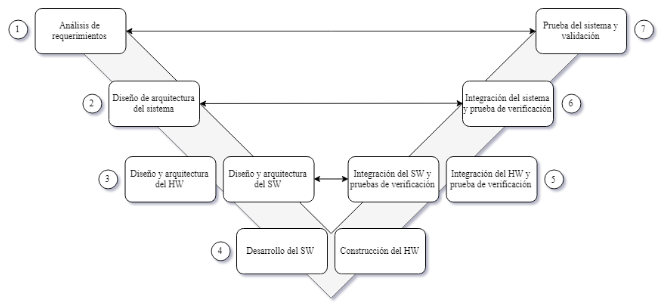
\includegraphics[width=\textwidth]{Introduccion/imagenes/metodologia.png}}
	\caption{Fases del modelo en V.}
	\label{fig:IntroduccionMetodologia}
\end{figure}

El desarrollo se llevará a cabo en las siguientes etapas:

\begin{enumerate}
	\item Análisis de requerimientos. Esta fase consiste en establecer qué debe hacer el sistema ideal, sin determinar cómo se construirá o diseñará el software. 
	\item Diseño de arquitectura del sistema. El diseño de la arquitectura del sistema consiste en varios pasos, como refinar las funciones del sistema y asignarlas a los diferentes componentes del sistema que pueden ser físicos o de hardware.
	\item Diseño de arquitectura de SW y HW. En esta fase del desarrollo del sistema, se diseña el hardware y el software de los diversos elementos que constituyen los componentes del sistema global. Las actividades que se aplican son similares a las realizadas en la fase anterior, pero centrándose en un componente específico del sistema: 
	\begin{itemize}
		\item Refinamiento de los requerimientos funcionales y no funcionales del hardware y software.
		\item Asignación de las funciones del software a los componentes de hardware.
	\end{itemize}
	\item Desarrollo del SW y Construcción del HW. Una vez que todos los componentes del sistema están diseñados, los elementos de hardware se construyen físicamente y los módulos de software son desarrollados en paralelo, y finalmente integrados con el hardware. Al final de este paso, los elementos de software y hardware deben estar disponibles para las actividades de verificación. Pueden realizarse algunas pruebas unitarias en paralelo con la implementación.
	\item Integración y verificación del SW y HW. En este paso se ensamblan los componentes de hardware y software. Las pruebas de verificación se ejecutan para comprobar el cumplimiento de los objetivos de diseño.
	\item Integración del sistema y prueba de verificación. En este paso, los elementos del sistema (HW, SW) se combinan y tiene lugar la verificación de los requisitos del sistema. 
	\item Prueba del sistema y validación. Esta última de verificación tiene como objetivo validar si los resultados obtenidos cumplen con los requerimientos.
\end{enumerate}